\documentclass[a4paper,12pt]{article}
\usepackage[utf8]{inputenc}
\usepackage[spanish]{babel}
\usepackage{microtype}

\usepackage{graphicx}
\usepackage{wrapfig}

\usepackage{amssymb}
\usepackage{amsmath} %For being able to make comments inside the formulas as normal text
\usepackage{amsthm}

\usepackage{cancel} %in the preamble gives you four different modes of striking through

\usepackage[a4paper, inner= 2cm, outer= 2cm,
top= 2cm, bottom= 2cm]{geometry}
\usepackage{fancyhdr}
\usepackage{animate}
\usepackage{hyperref}
\usepackage{float}
\usepackage[dvipsnames]{xcolor}
\definecolor{blueMacc}{RGB}{61, 160, 250}

\title{\textcolor{blueMacc}{Mergesort Paralelizada en c++}}
\author{David Alsina y Nicolás Quintero}
\date{Febrero 2021}



\begin{document}

    \begin{figure}[ht]
        \centering
        
\includegraphics[width = 17cm]{Header.png}
        \maketitle
    \end{figure}
    
    \href{https://github.com/juannico007/talleres_c.paralela.git}{\textcolor{blueMacc}{\underline{Github}}} 
    
    \section{Resumen}
    
    Para el desarrollo de este proyecto construimos el algoritmo \textit{mergesort} y lo paralelizamos usando la librería \textit{Open MP}
    \footnote{\href{https://www.openmp.org/}{\textcolor{blueMacc}{\underline{página de la organización}}}}
    \footnote{\href{https://medium.com/swlh/introduction-to-the-openmp-with-c-and-some-integrals-approximation-a7f03e9ebb65}{\textcolor{blueMacc}{\underline{artículo introductorio a \textit{open MP}}}}} y una modificación a este algortimo para incrementar el rendimiento \textit{(Se realiza un insertion sort cuando el tamaño del array llega a ser de 100 o menor)},
    adicionalmente para hacer posible el testeo de este algoritmo se usó computación en el cluster de la Universidad del Rosario \footnote{\textcolor{blueMacc}{\underline{\href{https://www.urosario.edu.co/}{Universidad del rosario}}}}, se hicieron pruebas desde la versión serial \textit{(un solo hilo)}, hasta 16 hilos, usando un incremento de 1 hilo en cada iteración. \textit{Los resultados se pueden ver a continuación.}
    
    \newpage
    
    \section{Resultados de Speedups}
    
    \begin{figure}[ht]
        \centering
        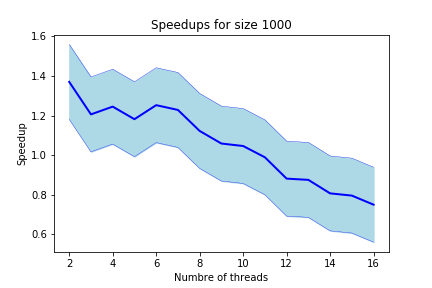
\includegraphics[width =0.55\linewidth]{Speedups for size 1000.png}
        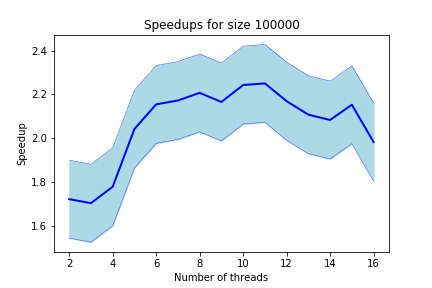
\includegraphics[width =0.55\linewidth]{Speedups for size 100000.png}
        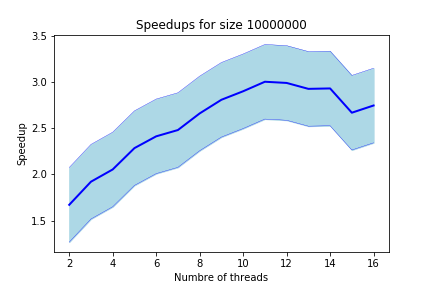
\includegraphics[width =0.55\linewidth]{Speedups for size 10000000.png}
    \end{figure}
    
    \begin{figure}[ht]
    \centering
        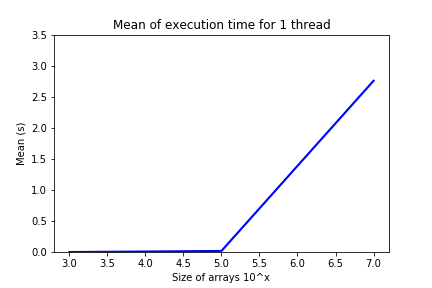
\includegraphics[width = 0.45\linewidth]{Mean of execution time for 1 thread.png}
        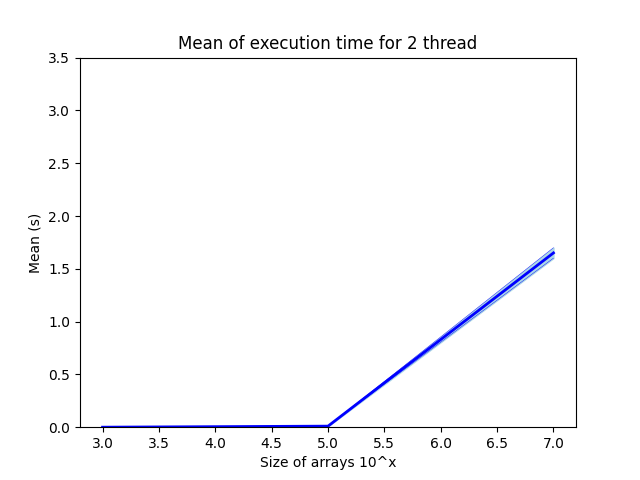
\includegraphics[width = 0.45\linewidth]{Mean of execution time for 2 thread.png}
        \includegraphics[width =     0.45\linewidth]{Mean of      execution time for 3         thread.png}
        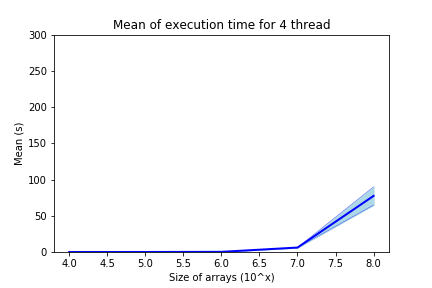
\includegraphics[width = 0.45\linewidth]{Mean of execution time for 4 thread.png}
        \includegraphics[width =     0.45\linewidth]{Mean of      execution time for 5         thread.png}
        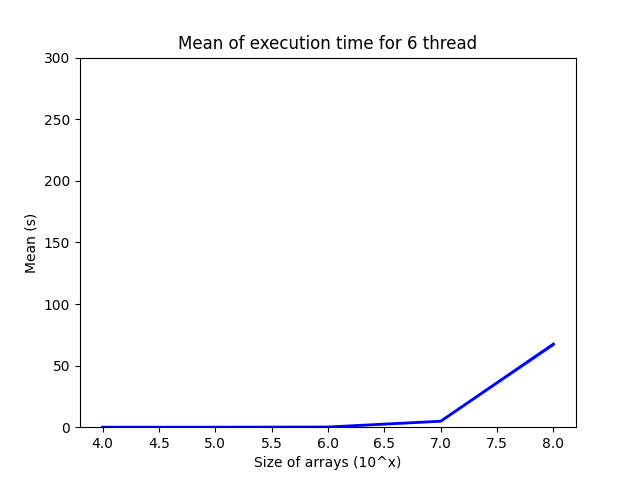
\includegraphics[width = 0.45\linewidth]{Mean of execution time for 6 thread.png}
        \includegraphics[width =     0.45\linewidth]{Mean of      execution time for 7         thread.png}
        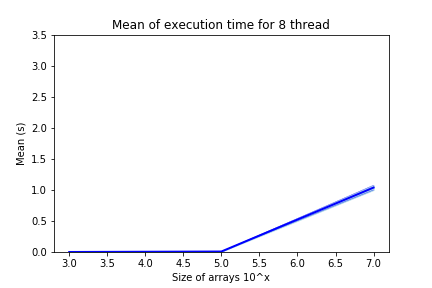
\includegraphics[width = 0.45\linewidth]{Mean of execution time for 8 thread.png}
    \end{figure}
    En el caso de arreglos de tamaño $10^3$ podemos observar que no se logra conseguir un speedup mayor a 1.4, y que a medida que el número de hilos aumenta, el speedup disminuye. Esto se debe a que el método utilizado para la paralelización del ordenamiento es tasking y al aumentar el número de hilos, el tiempo que tarda el hilo maestro en generar y asignar las tareas se vuelve mayor al tiempo que tarda el merge sort en ejecutarse sobre este tamaño del arreglo.
    
    Para los arreglos de tamaño $10^5$ y $10^7$ logramos observar que el número de hilos con el que obtuvo un mejor speedup fue de 11.
  
     
    \section{Resultados de promedios y desviaciones estándar por hilo}
    
    \begin{figure}[H]
    \centering
        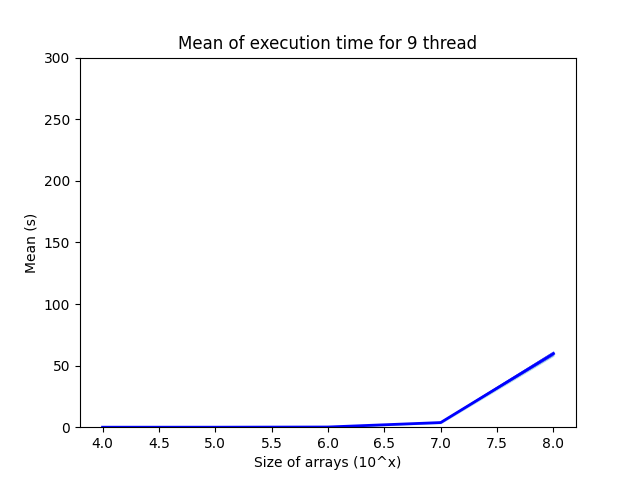
\includegraphics[width = 0.45\linewidth]{Mean of execution time for 9 thread.png}
        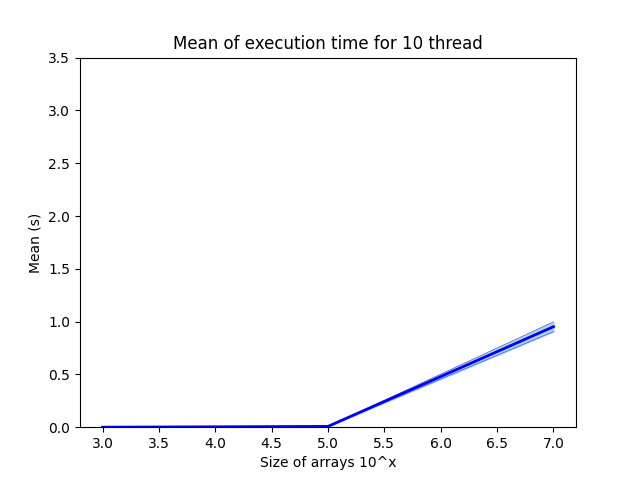
\includegraphics[width = 0.45\linewidth]{Mean of execution time for 10 thread.png}
        \includegraphics[width =     0.45\linewidth]{Mean of      execution time for 11         thread.png}
        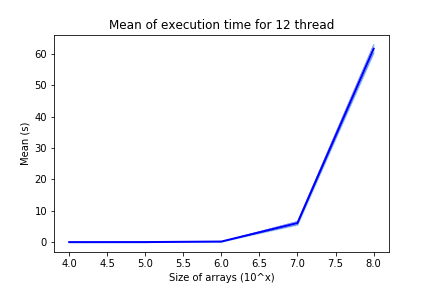
\includegraphics[width = 0.45\linewidth]{Mean of execution time for 12 thread.png}
        \includegraphics[width =     0.45\linewidth]{Mean of      execution time for 13         thread.png}
        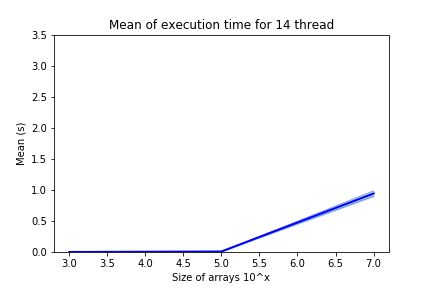
\includegraphics[width = 0.45\linewidth]{Mean of execution time for 14 thread.png}
        \includegraphics[width =     0.45\linewidth]{Mean of      execution time for 15         thread.png}
        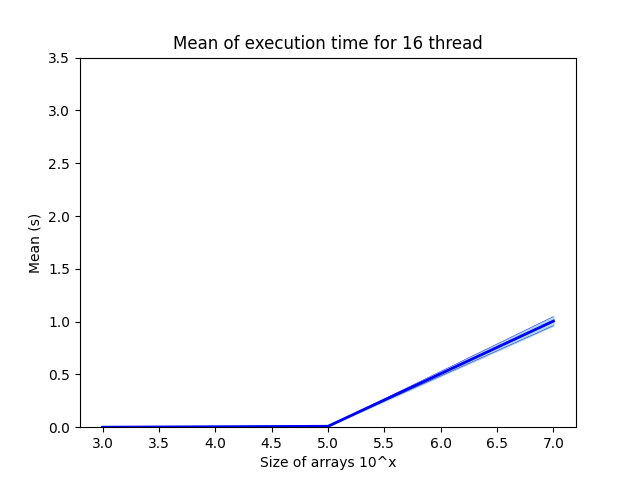
\includegraphics[width = 0.45\linewidth]{Mean of execution time for 16 thread.png}
    \end{figure}

\end{document}